\documentclass[tikz,10pt]{standalone}

\definecolor{ccred}{cmyk}{0, 0.87, 0.8, 0.21}

\begin{document}
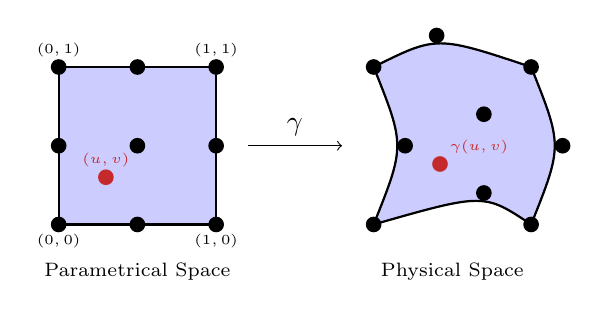
\begin{tikzpicture}[scale=2]

% Coordinates of the points to work
\coordinate (0) at (0,0);
\coordinate (1) at (1,0);
\coordinate (2) at (0,1);
\coordinate (3) at (1,1);
\coordinate (4) at (0.7,0.2);
\coordinate (5) at (0.2,0.5);
\coordinate (6) at (1.2,0.5);
\coordinate (7) at (0.4,1.2);
\coordinate (8) at (0.7,0.7);


% Parametrical Space
\draw [black, thick, fill=blue!20!white] (-2,0) -- (-1,0) -- (-1,1) -- (-2,1) -- (-2,0) ;
\draw (-2,0) node[circle,fill=black,inner sep=2pt] {} node[below] {\tiny $(0,0)$} ;
\draw (-1,0) node[circle,fill=black,inner sep=2pt] {} node[below] {\tiny $(1,0)$} ;
\draw (-1,1) node[circle,fill=black,inner sep=2pt] {} node[above] {\tiny $(1,1)$} ;
\draw (-2,1) node[circle,fill=black,inner sep=2pt] {} node[above] {\tiny $(0,1)$} ;

\draw (-1.5,0) node[circle,fill=black,inner sep=2pt] {};
\draw (-1.5,0.5) node[circle,fill=black,inner sep=2pt] {};
\draw (-1.5,1) node[circle,fill=black,inner sep=2pt] {};
\draw (-2,0.5) node[circle,fill=black,inner sep=2pt] {};
\draw (-1,0.5) node[circle,fill=black,inner sep=2pt] {};

% Blue background
\draw [black, thick, fill=blue!20!white] (0) .. controls (4) .. (1) .. controls (6) .. (3) .. controls (7) .. (2) .. controls (5) .. (0) ;

%%%%%%%%%% Link between control points %%%%%%%%%%
%\draw[color=black!40!white] (0) -- (4) -- (1) -- (6) -- (3) -- (7) -- (2) -- (5) -- (0) ;

%%%%%%%%%% Edges %%%%%%%%%%
\draw[color=black] (0) .. controls (4) .. (1) ;
\draw[color=black] (1) .. controls (6) .. (3) ;
\draw[color=black] (3) .. controls (7) .. (2) ;
\draw[color=black] (2) .. controls (5) .. (0) ;

% Plot the black nodes
% On Block Corners
\foreach \i in {0,...,3}
{
    \draw (\i) node[circle, fill=black, inner sep=2pt] {} ;
}
% On Block Edges
\foreach \i in {4,...,7}
{
    \draw (\i) node[circle, fill=black, inner sep=2pt] {} ;
}
% On Block Face
\draw (8) node[circle, fill=black, inner sep=2pt] {} ;


% Legend
\draw (-1.5,-0.3) node {\scriptsize Parametrical Space};
\draw (0.5,-0.3) node {\scriptsize Physical Space};
\draw[->] (-0.8,0.5) -- (-0.2,0.5) node[pos=0.5,above] {$\gamma$};

% Red dots
\draw (-1.7,0.3) node[circle, fill=ccred, inner sep = 2pt] {} node[above] {\tiny \textcolor{ccred}{$(u,v)$} };
\draw (0.42138,0.384) node[circle, fill=ccred, inner sep = 2pt] {} node[above right] {\tiny \textcolor{ccred}{$\gamma(u,v)$}};

\end{tikzpicture}
\end{document}